\documentclass[10pt,journal,compsoc]{IEEEtran}

\usepackage[pdftex]{graphicx}
\usepackage{cite}
\hyphenation{op-tical net-works semi-conduc-tor}


\begin{document}

\title{Using Deep Neural Networks for autonomus drone navigation in orchard enviroiment}

\author{BRESILLA, Trim}

\markboth{Inference project, Robotic Nanodegree, Udacity}%
{}
\IEEEtitleabstractindextext{%

\begin{abstract}
    With the increase of population in the world, the demand for quality food is increasing too. One of the biggest and the base of raw food production comes frim Agriculture. In the recent years, due to this demand, and other enviroimental factors have havily influenced the way agricultural production is done. Automation and robotics for fruit and vegetable production and monitoring has become the new standard. In this /paper/ we disscus an autonomus drone that would be bale to navigate through the rows in an onrchard enviroiment. The drone is made of a flight controller (PixHawk), an micorocntroller (Aarduino) for analog reading from differnet sensors, and a on-board computer (Raspberry Pi gen. 3). Pictres are taken through PiCamera and streamed through WiFi to a computer running a neaurl network model. Based on prior trainings, the moderunning a neaurl network model. Based on prior trainings, the model sents back the direction to the drone, thus performing navigation.
\end{abstract}

\begin{IEEEkeywords}
Robotics, Agriculture, Udacity, Orchard, Deep Learning.
\end{IEEEkeywords}}


\maketitle
\IEEEdisplaynontitleabstractindextext
\IEEEpeerreviewmaketitle
\section{Introduction}
\label{sec:introduction}

\IEEEPARstart{A}{utomation} in Agriculture is recent years i highly increasing. Eventhough Agriculture as one of the oldest occupation in the world, has seen many changes during centuries. Before Industrial Revolution was estimated that more than 80\% of population were working as farmers, while now is estimated that number to be 2\%. One of the dominant changes that characteries a growing economy is the proportionate decline in Agriculture Sector. This phenomenon is commonly atributed to two facts: food is not as demnading as other goods and services, and the rapid development of new farming technologies lead to expanding food supplies per hectare and per worker.
%IMAGE
\begin{figure}[thpb]
      \centering
      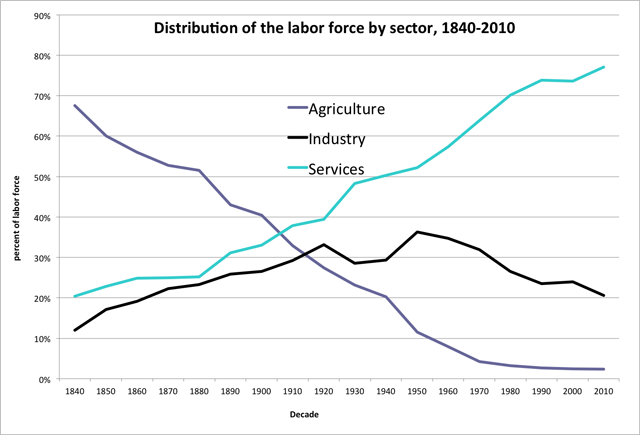
\includegraphics[width=\linewidth]{agridecline}
      \caption{Industrial Revolution.}
      \label{fig:robot1}
\end{figure}

The decrease shows significance every step of the industrial revolution. Industry 1.0 brought mechanisation, water management etc.; Industry 2.0 brought steam engines, electricity, protected enviroiments etc.; Industry 3.0 broight computers and smart apliances, GPS trctors and so on; while Industry 4.0 is foreseen to be the most significant one, bringing AI, Automation and Robotics.

The chanllenge of how we'll feed the evergrowing world populatoin in the future - is sustainable, cost-effective anf most importantly enviroimentally friendly. In order to feed 9.5 billion people that Food and Agriculture Organisation (FAO) predicts to inhabit the planet by 2050 while climate change is making more dificult to grow crops - is going to be done by Smart Farming, a high-tech and AI driven agricultural management system. Agriculture is highly repetitive, and such, many tasks can and are being automated. Robots/AI would improve production yeild while reducing resources required by making precision sequence of actions.

For crop farming, robots need to autonomously navigate their environment and perform actions at set locations, for example, picking a fruit, spraying a pesticide, planting a seed, imaging a plant, or making a measurement. Glasshouses are slightly simpler to move around since the environment is more carefully engineered, and is often fit with tracks which robots follow to reach desired locations. In the case of outdoor farming, the robots work by receiving a plan with a set of locations to visit on the field. When the robot trajectories are known, the robot can use GPS positioning and a closed-loop control to make sure it remains on track. When the task is to follow an unknown trajectory, for example a crop row, vision is often used to allow the robot to find its way. Robots are wirelessly connected to a central operator to both receive updated instructions regarding the mission, and report status and data. Put together, making an autonomous farm robot requires clever controllers, localisation and communication systems. To a certain extent, the technology is similar to that of autonomous cars applied to agtech. Where it differs is that farming robots often need to manipulate their environment, picking vegetables or fruits, applying pesticides in a localised manner, or planting seeds. All these tasks require sensing, manipulation, and processing of their own. 

\section{Background / Formulation}

\section{Data Acquisition}

\section{Results}

\section{Discussion}

\section{Conclusion / Future work}

\bibliography{bib}
\bibliographystyle{ieeetr}

\end{document}
